\documentclass[10pt,twocolumn]{article}
\usepackage[a4paper,margin=16mm,columnsep=6mm]{geometry}
\usepackage{amsmath,amssymb}
\usepackage{booktabs}
\usepackage{graphicx}
\usepackage{microtype}
\usepackage{xcolor}
\usepackage{hyperref}
\usepackage{caption}
\usepackage{subcaption}
\usepackage{enumitem}
\usepackage{array}
\usepackage{tabularx}
\usepackage{multicol}
\usepackage{tikz}
\usetikzlibrary{arrows.meta,positioning,fit}
\hypersetup{colorlinks=true,linkcolor=teal!55!black,citecolor=teal!55!black,urlcolor=teal!55!black}
\graphicspath{{figures/}}
\captionsetup{font=small,labelfont=bf}
\setlist{nosep,leftmargin=*}
\setlength{\parindent}{1em}
\setlength{\parskip}{0.25em}

\definecolor{mixed}{HTML}{0F766E}
\definecolor{pure}{HTML}{2563EB}
\definecolor{strict}{HTML}{EA580C}
\definecolor{ink}{HTML}{172033}

\title{\vspace{-1.2em}\textbf{Chasing the Nines: Reliability Across States and Seeds}\\[-1mm]\large A Fixed-Grid Pendulum Case Study}
\author{Ala Sleimi \and \href{https://www.moodle.tum.de/user/view.php?id=261287\&course=117206}{Mykhailo Shtandenko}\\
\small Supervisor: \href{https://www.moodle.tum.de/user/view.php?id=140042\&course=117206}{Lennart R\"ostel}}
\date{30 July 2026}

\begin{document}
\maketitle
\vspace{-1.5em}

\begin{abstract}
A control policy is only useful if it generalizes across both initial
conditions and the randomness introduced by different training seeds.
To test this, we compare five trained actors on an identical grid of
2{,}501 states in the Pendulum environment.

Among the candidates, the best-performing pipeline that combines
reinforcement learning with supervised guidance succeeds close to the
reference trajectory in 12{,}496 out of 12{,}505 seed-state trials,
corresponding to a success rate of 99.928\%. By contrast, the strongest
pure reinforcement-learning pipeline succeeds in 12{,}008 trials
(96.026\%). Looking specifically at task completion, the two pipelines
achieve success rates of 93.858\% and 92.875\%, respectively; however,
the pure-RL policy more frequently matches the reference solution
exactly, winning strictly in 22.823\% of cases compared to 12.555\%
for the hybrid pipeline.

Examining failures more closely, the pure-RL actor fails in 1{,}267
instances. Of these, applying reflection combined with an exhaustive
search over the critic's full range of admissible actions is able to
correct 770 cases. The unresolved failures point to two distinct but
related issues. First, when reference actions are applied in sequence,
only 19.1\% of failures are corrected after a single corrective action,
while 99.0\% are resolved after a sequence of 32 actions — indicating
that recovery from failure typically requires a coordinated,
multi-step correction rather than a single fix. Second, an analysis of
the FastSACN8 actors shows that 98.5\% of their failed actions lie near
the boundary of the allowable torque range; once clipped to this
boundary, only 7.1\% of the locally optimal critic-suggested
adjustment is actually retained. This finding motivates searching over
the entire torque interval rather than relying on local adjustments
alone.

Taken together, these results suggest that pure reinforcement learning
by itself is unlikely to reach the desired reliability threshold. They
point instead toward a promising direction for future work: combining
supervised pre-training, reward-driven RL fine-tuning, and an inductive
bias grounded in the system's underlying symmetry.
\end{abstract}

\section{Reliability target and evidence}

\paragraph{Chasing two kinds of nines.}
The project asks how to increase reliability within one trained model and across random training seeds. A high pooled score can conceal different failures in different seeds. Every mainline method is therefore evaluated on 61 angles in $[-\pi,\pi]$ and 41 angular velocities in $[-1,1]$. Five actor seeds yield 12,505 deterministic 200-step rollouts in Gymnasium \texttt{Pendulum-v1}.

The observation, torque, and reward are
\[
s=(\cos\theta,\sin\theta,\dot\theta),\quad a\in[-2,2],
\]
\[
r_t=-(\theta_t^2+0.1\dot\theta_t^2+0.001a_t^2).
\]
The scoring reference is the better stored return from a dynamic-programming policy and a controller,
$R^\star(s)=\max(R_{\rm DP}(s),R_{\rm ctrl}(s))$.

For policy return $R_\pi(s)$, near-reference and strict-win indicators are
\[
\begin{aligned}
\mathcal N(s)&=\mathbb 1[R_\pi(s)\ge R^\star(s)-5],\\
\mathcal B(s)&=\mathbb 1[R_\pi(s)>R^\star(s)].
\end{aligned}
\]
Task success requires upright conditions on at least 80\% of steps and limits every consecutive interval outside that region to 50 steps. A step is near upright when $\cos\theta\ge0.95$ and $|\dot\theta|\le1$.

\paragraph{Evaluation design.}
Every headline row uses the common grid, five independently trained actors, and at most 100,000 learning transitions in each selected pipeline. Every displayed scorecard therefore contains 12,505 rollouts. The mixed pipeline uses reference actions during training and deploys learned actor and critic networks. The scorecard evaluates both selected pipelines on one fixed test; Table~\ref{tab:resources} reports their resource use.

 \paragraph{Prior work and design hypotheses.}
Our approach draws on several existing techniques. Soft Actor-Critic
(SAC) learns a stochastic policy together with two critic networks by
optimizing a combination of expected reward and entropy
\cite{haarnoja2018sac}; SimbaV2 builds on this by introducing
normalized residual architectures that improve the stability of deep
RL training \cite{lee2025simba}. Together, these form our reward-only
baseline. Separately, DAgger addresses distribution shift over the
course of a trajectory by relabeling states the learner actually
visits \cite{ross2011dagger}; we extend this idea by automatically
prioritizing initial states with the highest measured regret, in the
spirit of prioritized-curriculum methods \cite{jiang2021plr}. To handle
longer-horizon credit assignment, SACn incorporates multi-step return
losses, importance weighting, and a lower-variance entropy estimator
\cite{lyskawa2025sacn}. Building on this, our SACN8 variant considers
horizons ranging from one to eight steps, and a lighter version,
FastSACN8, retains only the one-step and eight-step endpoints.

For action selection, we adopt the general principle of critic-guided
action search \cite{kalashnikov2018qtopt}, extending it with a fixed
set of candidate actions and a requirement that both critics agree
before an action is accepted. In addition, we incorporate a reflection
step that exploits the known sign symmetry inherent to the Pendulum
task. Because average performance metrics can mask underlying
instability, we adopt multi-seed evaluation throughout, consistent
with recommendations from prior work on reproducibility in RL
\cite{henderson2018matters,agarwal2021precipice}.

Building on these components, our study assembles two full pipelines,
evaluates the contribution of each retained component using paired
seed-state trials, and investigates why the pure-RL pipeline exhibits
a higher failure rate. In particular, we examine three questions:
whether successful recovery from failure requires multiple coordinated
corrective actions, whether the critic is able to identify useful
alternative actions in the first place, and whether the actor's
bounded output range is expressive enough to realize those corrections.

\clearpage
\onecolumn
\small
\section{The two selected recipes}
\vspace{2mm}

\begin{center}
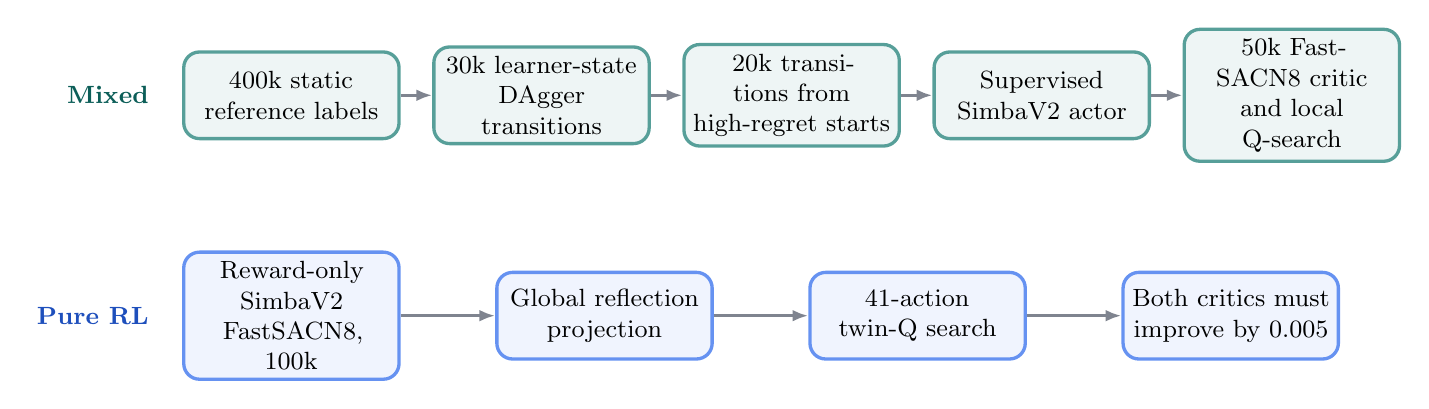
\begin{tikzpicture}[
  node distance=5mm and 4mm,
  every node/.style={font=\small,align=center},
  box/.style={rounded corners=2mm,very thick,minimum height=11mm,text width=25mm},
  mixedbox/.style={box,draw=mixed!70,fill=mixed!7},
  purebox/.style={box,draw=pure!70,fill=pure!7},
  arrow/.style={-{Latex[length=2mm]},very thick,draw=ink!55}
]
\node[mixedbox] (mstatic) {400k static\\reference labels};
\node[mixedbox,right=of mstatic] (mdagger) {30k learner-state\\DAgger transitions};
\node[mixedbox,right=of mdagger] (mpriority) {20k transitions from\\high-regret starts};
\node[mixedbox,right=of mpriority] (mactor) {Supervised\\SimbaV2 actor};
\node[mixedbox,right=of mactor] (mlocal) {50k FastSACN8 critic\\and local Q-search};
\draw[arrow] (mstatic) -- (mdagger);
\draw[arrow] (mdagger) -- (mpriority);
\draw[arrow] (mpriority) -- (mactor);
\draw[arrow] (mactor) -- (mlocal);

\node[purebox,below=14mm of mstatic] (psac) {Reward-only SimbaV2\\FastSACN8, 100k};
\node[purebox,right=12mm of psac] (preflect) {Global reflection\\projection};
\node[purebox,right=12mm of preflect] (pq) {41-action\\twin-Q search};
\node[purebox,right=12mm of pq] (paccept) {Both critics must\\improve by 0.005};
\draw[arrow] (psac) -- (preflect);
\draw[arrow] (preflect) -- (pq);
\draw[arrow] (pq) -- (paccept);

\node[font=\bfseries\small,text=mixed!80!black,left=3mm of mstatic] {Mixed};
\node[font=\bfseries\small,text=pure!80!black,left=3mm of psac] {Pure RL};
\end{tikzpicture}
\captionof{figure}{The mixed actor receives direct actions on the states it visits, then a reward critic makes small local corrections. Pure RL learns from reward, imposes the Pendulum symmetry, and searches a wider action set with its critics.}
\label{fig:recipes}
\end{center}

\vspace{1mm}
\begin{multicols}{2}
\paragraph{Mixed recipe in plain language.}
The pipeline begins with a SimbaV2 actor, using two residual blocks of
width 64, that first learns to imitate reference actions. Following
this initial phase, three rounds of DAgger allow the actor to actually
control the pendulum, with each round labeling whichever states the
actor visits under its own control. In the subsequent refinement step,
we sample starting states uniformly, rank them according to their
measured regret, and draw an additional 20{,}000 transitions—drawing
predominantly from the weakest starting states, supplemented by a
uniformly sampled fraction. As a result, the training set comes to
include states that only arise after the actor has already made
earlier mistakes.

For the initializer, we train on 400k examples for 80 epochs using a
batch size of 1{,}024 and a learning rate of $3{\times}10^{-4}$. Each
subsequent DAgger round contributes 10k additional transitions from
the learner, and the final high-regret refit is performed over three
epochs with a reduced learning rate of $10^{-5}$.

The supervised actor is trained by minimizing the behavior-cloning loss
\[
\mathcal L_{\rm BC}(\theta)=
\frac{1}{|\mathcal D|}\sum_{(s,a^\star)\in\mathcal D}
\left(\frac{\pi_\theta(s)-a^\star}{2}\right)^2.
\]

Separately, a categorical FastSACN8 critic—also width 64 with two
residual blocks, and shared across both pipelines—is trained purely
from reward signal, using a batch size of 256 and two gradient updates
per transition.

At deployment time, the actor first proposes an action
$a_0=\pi_\theta(s)$. The critic then evaluates a small neighborhood of
candidate perturbations around this proposal:
\[
\mathcal A_{\rm local}=
\operatorname{clip}\!\left(a_0+\{-0.10,-0.05,0,0.05,0.10\},-2,2\right).
\]
The original proposal $a_0$ is only replaced by the highest-valued
alternative when both critics independently agree that it is
preferable.

Finally, the categorical critic's loss function combines two
cross-entropy terms, corresponding to one-step and eight-step returns.
With weighting $w_n=\lambda^{n-1}$ and $\lambda=0.5$, the normalized
weight assigned to the eight-step term works out to
\[
\frac{0.5^7}{1+0.5^7}=0.775\%.
\]

\paragraph{Pure-RL recipe in plain language.}
We now describe the pure-RL configuration in detail. Five independent
SimbaV2 actor-critic agents were trained from scratch, each for
100{,}000 environment transitions, using only the reward signal with
no supervisory guidance. The actor network is kept intentionally
compact, consisting of a single residual block of width 32. The twin
categorical critics, by contrast, are somewhat larger: each has two
residual blocks, a width of 64, and represents its value distribution
using 51 return atoms \cite{bellemare2017distributional}.

Whereas conventional Soft Actor-Critic bootstraps from a single step,
our design targets longer-horizon credit assignment. The SACN8
variant computes losses jointly across every horizon from one to
eight steps; a faster alternative, FastSACN8, reduces this to just the
one-step and eight-step losses in order to lower computational cost
while preserving most of the benefit. In the final selected
configuration, the eight-step loss is down-weighted by a factor of
$\lambda^7$, and each critic receives two gradient updates per
environment transition. At deployment time, we apply a symmetry
correction to smooth over inconsistencies in the actor's behavior, and
additionally use a Q-search step to propose alternative actions—though
conservatively, replacing the actor's default choice only when both
critics agree the alternative is better.

As in standard SAC, the actor is trained to minimize
$\mathbb E[\alpha\log\pi_\theta(a|s)-\min_iQ_i(s,a)]$. For the critic
update, let $Y_t^{(n)}$ denote the $n$-step soft return and $Z_t^{(n)}$
its categorical projection. For horizon $n\in\{1,8\}$, the return is
given by:
$$\begin{aligned}
Y_t^{(n)}={}&\sum_{j=0}^{n-1}\gamma^j
\left(r_{t+j}+\gamma\alpha\widehat H_n(\pi(\cdot|s_{t+j+1}))\right)\\
&+\gamma^n\min_i\bar Q_i(s_{t+n},a'),\qquad a'\sim\pi(\cdot|s_{t+n}).
\end{aligned}$$

Writing $\operatorname{CE}(Z,Q_i)$ for the cross-entropy between this
projected target and the $i$-th critic's predicted distribution,
FastSACN8 minimizes the combined objective:
$$\mathcal L_Q=
\frac{1}{1+\lambda^7}
\sum_{i=1}^{2}\mathbb E\!\left[
\operatorname{CE}\!\left(Z^{(1)},Q_i\right)+
\lambda^7\operatorname{CE}\!\left(Z^{(8)},Q_i\right)
\right].$$

All results are reported across five seeds, numbered 0 through 4.
Networks are optimized with Adam using a batch size of 256, a replay
buffer holding up to 100k transitions, a discount factor of
$\gamma=.99$, and a soft target-update rate of $\tau=.005$. Learning
rates for both actor and critic decay linearly from $10^{-4}$ to
$5{\times}10^{-5}$ over training. Once training begins, each
environment transition triggers two critic updates and one actor
update.

During deployment on the Pendulum task, we exploit the environment's
sign symmetry to stabilize the policy's behavior. Defining the
symmetric state transformation $M(s)$ and the corresponding
symmetrized action $a_{\rm sym}(s)$:
$$\begin{aligned}
M(s)&=(\cos\theta,-\sin\theta,-\dot\theta),\\
a_{\rm sym}(s)&=\frac{\pi_\theta(s)-\pi_\theta(M(s))}{2}.
\end{aligned}$$

After this symmetrization step, the Q-search procedure evaluates 41
evenly spaced candidate torques spanning $[-2,2]$ using the learned
critics, selecting the top-scoring option
$a_q=\arg\max_a\min_iQ_i(s,a)$. This candidate is only adopted in
place of the symmetrized action if it offers a clear, reliably
predicted improvement—specifically, both critics must indicate an
advantage exceeding 0.005:
$$Q_i(s,a_q)-Q_i(s,a_{\rm sym})>0.005
\quad\text{for }i\in\{1,2\}.$$

\paragraph{Resource accounting.}
The chosen hybrid pipeline draws on 30k DAgger transitions collected
from learner-visited states, 20k additional transitions from
high-regret states, and a single shared critic trained on 50k
transitions—yielding 100k total learning transitions. Its reference
labeling requirements total 690k queries, broken down into 400k labels
for the initializer, 30k for learner-state DAgger, 240k for
reset-support states, and 20k for high-regret refinement. An
additional 800k candidate-rollout interactions are used solely to rank
candidate starting states. Because the 50k-transition critic is shared
across all five actors, the hybrid study as a whole uses 300k learning
transitions in total. The pure-RL approach, by comparison, uses 100k
learning transitions per seed, totaling 500k across the five complete
actor-critic runs. Notably, both selected pipelines rely on 100k
learning transitions per individual trained deployment; full
study-wide totals are summarized in Table~\ref{tab:resources}.

\begin{center}
\footnotesize
\captionof{table}{Learning, search, and reference-data resources. Each selected deployment uses 100k learning transitions.}
\label{tab:resources}
\begin{tabularx}{\columnwidth}{@{}Xrr@{}}
\toprule
Resource & Mixed & Pure RL\\
\midrule
Learning transitions per deployment & 100k & 100k\\
Learning transitions in full study & 300k & 500k\\
Start-ranking rollout interactions & 4.00m & 0\\
Reference labels in full study & 3.45m & 0\\
\bottomrule
\end{tabularx}
\end{center}
\end{multicols}

\normalsize
\clearpage
\onecolumn
\section{Reliability and component results}

\begin{center}
\includegraphics[width=.68\textwidth]{37_core_scorecard_large.png}
\captionof{figure}{Scorecard on the same 12,505 seed-state trials. Every row uses five actors; the mixed rows share one selected critic.}
\label{fig:scorecard}
\end{center}

\vspace{-1mm}
\begin{minipage}[t]{.49\textwidth}
\centering
\includegraphics[width=.98\linewidth]{77_failure_footprints_stacked_axes.png}
\captionof{figure}{Failure footprints on the common evaluation grid. Color counts failed actor seeds at each initial state: light cyan, yellow, orange, red, and black denote one through five failures.}
\label{fig:footprints}
\end{minipage}\hfill
\begin{minipage}[t]{.48\textwidth}
\footnotesize
\paragraph{The mixed method fails on only nine trials.}
Out of 12,505 near-reference trials, the selected mixed pipeline
succeeds on 12,496, compared with 12,008 for the pure-RL pipeline
(Figure~\ref{fig:scorecard}). Task-level success is recorded in 11,737
cases for the mixed pipeline versus 11,614 for pure RL, while pure RL
achieves strict wins more often—2,854 compared with 1,570. The two
pipelines therefore rank differently depending on whether the metric
of interest is reliability or exceeding the stored comparator.

\paragraph{The gap is seed-dependent.}
Per-seed near-reference counts for the mixed pipeline range from 2,494
to 2,501 out of 2,501 states, whereas pure RL ranges from 2,333 to
2,457. Task-success and strict-win counts for the mixed pipeline span
2,342--2,354 and 254--419 respectively; for pure RL, these ranges are
2,310--2,338 and 532--605. All five seeds succeed together on 2,493
cells for the mixed pipeline (99.680\%). By contrast, pure RL succeeds
across all five seeds on only 2,293 cells, fails across all five on
13, and shows seed-dependent variability on the remaining 195 cells.
Figure~\ref{fig:footprints} illustrates this contrast: the mixed
pipeline's failures form a small, isolated set, whereas pure RL shows
broader regions where multiple seeds fail simultaneously.
\end{minipage}

\vspace{4mm}
\begin{minipage}[t]{.47\textwidth}
\centering
\footnotesize
\captionof{table}{Mixed-pipeline near-reference failures on the common evaluation grid.}
\label{tab:mixed-ablation}
\begin{tabular}{lr}
\toprule
Deployment/training variant & Failures\\
\midrule
Full mixed pipeline & \textbf{9}\\
Uniform follow-up starts & 19\\
No local Q-search & 35\\
No learner-state labels & 38\\
\bottomrule
\end{tabular}

\vspace{1mm}
\footnotesize\raggedright
Including learner-state labels eliminates 29 failures, automatic
prioritization removes ten more beyond that, and conservative local
Q-search accounts for a further 26. Together, these matched variants
isolate the contribution of each component retained in the mixed
pipeline.
\end{minipage}\hfill
\begin{minipage}[t]{.47\textwidth}
\centering
\footnotesize
\captionof{table}{Pure-RL cumulative repair on the common evaluation grid.}
\label{tab:pure-ablation}
\begin{tabular}{lrr}
\toprule
Deployment rule & Failures & Repaired\\
\midrule
Raw actor & 1,267 & ---\\
$+$ reflection & 955 & 312\\
$+$ twin-critic Q-search & \textbf{497} & 458\\
\midrule
Total repaired & & \textbf{770}\\
\bottomrule
\end{tabular}

\vspace{1mm}
\footnotesize\raggedright
Together, reflection and Q-search resolve 60.8\% of the raw actor's
failures. The paired grid results demonstrate that the critics are
capable of assigning higher value to corrective actions even in cases
where the deterministic actor itself proposes a failing action.
\end{minipage}

\clearpage
\onecolumn
\section{Why sequence-aware training still needs full-range action search}

\begin{center}
\centering
\includegraphics[width=.98\textwidth]{58_poster_target_family_internals_wide.png}
\captionof{figure}{Completed 100k SimbaV2 configurations with five seeds each. Panels A and B use 5,553 fixed states per seed and show torque-bound occupancy and remaining tanh slope. Panels C and D use 512 fixed failure states per seed. C measures critic-preferred moves that improve realized return (blue), helpful reference actions ranked above actor actions (green), and projected moves that reduce return (orange). D shows bound occupancy (gray), critic requests farther outside the allowed interval (blue), and the local step preserved after clipping (orange).}
\label{fig:target-diagnostics}
\end{center}

\vspace{-1mm}
\begin{multicols}{2}
\small
\paragraph{Recovery spans several coordinated decisions.}
For each of the 1,267 raw-actor failures listed in
Table~\ref{tab:pure-ablation}, we substitute reference actions for the
first $K$ decisions before allowing the frozen actor to resume
control. The repair rate climbs steadily with $K$: from 19.1\% at
$K=1$ up to 47.7\%, 91.3\%, and finally 99.0\% at $K=8,16,32$.
Notably, shuffling that same sequence of 32 actions repairs only 0.6\%,
confirming that the order of corrective actions matters. This
dependence on an extended, ordered recovery horizon is precisely what
motivates sequence-aware critic targets—SACN8 trains across horizons
one through eight, while FastSACN8 retains only the one-step and
eight-step endpoints for efficiency.

\paragraph{Multi-step critics choose better local directions while their actors push harder against torque limits.}
Figure~\ref{fig:target-diagnostics} compares the fully trained
five-seed configurations. Compared to one-step SAC, both FastSACN8 and
SACN8 substantially increase the median share of actions sitting near
a torque limit, from 59.1\% up to 86.9\% and 86.7\% respectively. A
small step in the critic's preferred direction yields improved
realized return on 73.1\% of one-step states, rising to 74.8\% for
FastSACN8 and 76.2\% for SACN8. Meanwhile, the fraction of harmful
projected moves declines from 27.8\% to 26.6\% and 24.6\%. In short,
the multi-step critics identify marginally better local directions,
even as their corresponding actors leave increasingly little room to
act on them.

\paragraph{High actor torque motivates full-range Q-search.}
Among the examined failure states, actions lie within 0.05 of a
torque bound in 91.5\% of cases for one-step SAC, 98.5\% for
FastSACN8, and 98.9\% for SACN8. Their respective critics request a
move further outward in 82.0\%, 94.6\%, and 95.1\% of these states.
However, clipping preserves only 28.2\%, 7.1\%, and 6.9\% of a nominal
0.05-magnitude move—meaning small local adjustments have almost no
effect on failed FastSACN8 actions in particular. This is precisely
why the 41-action search spans the entire $[-2,2]$ interval, allowing
it to alter both the sign and magnitude of the torque.

\paragraph{Why Q5 for mixed and Q41 for pure.}
Across 27,765 fixed diagnostic trials, the mixed pipeline reaches
27,751 near-reference successes using Q5 search, compared to 26,975
using Q41. For pure RL, with reflection and the 0.005 agreement
threshold held fixed, Q5 search yields 25,657 successes (92.408\%)
while Q41 yields 26,629 (95.909\%)—an additional 972 successes. Notably,
Q5 alters only 690 out of 5,553,000 mixed-policy decisions (0.012\%).
This asymmetry reflects the fact that mixed actors already track the
reference action closely, whereas the more saturated pure actors
benefit substantially from candidates spanning a wider range of torque
sign and magnitude.

\paragraph{Both critics must agree before deployment changes an action.}
Looking at the first point of disagreement between actor and
reference, substituting the reference action improves the subsequent
return in 79.4\% of FastSACN8 failures. Among these helpful
substitutions, the learned critic assigns a higher Q-value to the
reference action in 54.5\% of cases. For one-step SAC and SACN8, this
figure rises to 86.4\% and 80.4\% respectively. In deployment, a
searched action is only accepted in place of the actor's proposal when
both critics agree it merits a value at least 0.005 higher.

\paragraph{FastSACN8 improves the deployed result through its critic.}
Across the same 27,765 fixed diagnostic trials, one-step actors reach
91.864\% near-reference success prior to any search, while the
selected FastSACN8 actors reach a somewhat lower 89.937\%. However,
once the same reflection and Q41 search rule are applied, these
figures rise to 94.489\% and 95.909\%, respectively. The selected
FastSACN8 configuration additionally uses $\lambda=0.5$ and two critic
updates per transition, and its advantage emerges specifically when
the critics are given the opportunity to choose among candidate
torques at deployment time. Interestingly, reflection benefits pure RL
but slightly hurts the mixed pipeline: adding it before mixed Q5
search reduces near-reference success from 27,751 to 27,749, which is
why the mixed deployment omits this step.

\paragraph{Standard-MLP target-family check.}
As a control, the standard-MLP experiment omits SimbaV2 entirely across
all three configurations, using 100k transitions with a single update
per transition. Actor-only near-reference reliability reaches only
8,243 of 12,505 trials for SAC (65.918\%), improving to 9,124 for
FastSACN8 (72.963\%) and 9,189 for SACN8 (73.483\%). Plain SAC clearly
lags behind both multi-step target variants; corresponding task-success
and strict-win figures are reported in the annex.

\paragraph{Conclusion and recommended recipe.}
Overall, the comparison clearly favors the mixed pipeline: just nine
failures across eight initial states, versus 497 failures across 208
states for the selected pure-RL pipeline. This strongly suggests that
pure RL alone is insufficient to meet the target reliability standard.
Learner-state labels alone eliminate 29 mixed-pipeline failures, while
for pure RL, reflection resolves 312 failures and Q-search resolves a
further 458 whenever both critics concur on a higher-valued action.
During the ADLR presentation, a tutor proposed an even stronger
symmetry-based experiment: training on only one symmetric half of the
state space and obtaining the other half purely through reflection. We
recommend testing this inductive bias by combining supervised
pre-training—on both reference and learner-visited states—with
subsequent reward-based RL refinement. This concrete recipe represents
the clearest hypothesis for closing the remaining gap to the next nine
failures.
\end{multicols}

\clearpage
\onecolumn


\clearpage
\begin{multicols}{2}
\begin{thebibliography}{10}
\bibitem{haarnoja2018sac}
T. Haarnoja, A. Zhou, P. Abbeel, and S. Levine.
\newblock Soft Actor-Critic: Off-policy maximum entropy deep reinforcement learning with a stochastic actor.
\newblock \emph{ICML}, 2018.

\bibitem{bellemare2017distributional}
M. Bellemare, W. Dabney, and R. Munos.
\newblock A distributional perspective on reinforcement learning.
\newblock \emph{ICML}, 2017.

\bibitem{ross2011dagger}
S. Ross, G. Gordon, and D. Bagnell.
\newblock A reduction of imitation learning and structured prediction to no-regret online learning.
\newblock \emph{AISTATS}, 2011.

\bibitem{jiang2021plr}
M. Jiang, E. Grefenstette, and T. Rockt\"{a}schel.
\newblock Prioritized level replay.
\newblock \emph{ICML}, 2021.

\bibitem{rajeswaran2018dapg}
A. Rajeswaran et al.
\newblock Learning complex dexterous manipulation with deep reinforcement learning and demonstrations.
\newblock \emph{RSS}, 2018.

\bibitem{kalashnikov2018qtopt}
D. Kalashnikov et al.
\newblock QT-Opt: Scalable deep reinforcement learning for vision-based robotic manipulation.
\newblock arXiv:1806.10293, 2018.

\bibitem{lee2025simba}
H. Lee, Y. Lee, T. Seno, D. Kim, P. Stone, and J. Choo.
\newblock Hyperspherical normalization for scalable deep reinforcement learning.
\newblock \emph{ICML}, 2025.

\bibitem{lyskawa2025sacn}
J. {\L}yskawa, J. Lewandowski, and P. Wawrzy{\'n}ski.
\newblock SACn: Soft Actor-Critic with n-step returns.
\newblock arXiv:2512.13165, 2025.

\bibitem{henderson2018matters}
P. Henderson et al.
\newblock Deep reinforcement learning that matters.
\newblock \emph{AAAI}, 2018.

\bibitem{agarwal2021precipice}
R. Agarwal, M. Schwarzer, P. Castro, A. Courville, and M. Bellemare.
\newblock Deep reinforcement learning at the edge of the statistical precipice.
\newblock \emph{NeurIPS}, 2021.

\end{thebibliography}
\end{multicols}

\ifdefined\REPORTBODYONLY
\else
\clearpage
\appendix
\onecolumn
\section{Evidence and diagnostics annex}
\small

\subsection{Evaluation protocol}

Each headline percentage comes from five trained actors evaluated on the same 61 by 41 grid. The diagnostic experiments reuse those actors on fixed state sets to examine the observed failure patterns.

The mixed actor family uses DAgger followed by 20,000 additional transitions from automatically selected high-regret starts. The pure deployment combines SimbaV2 FastSACN8 actors, symmetry projection, and a 41-candidate search that accepts a change only when both critics favor it. Both evaluations contain five actors and 12,505 common-grid rollouts.

The mixed initializer used 400,000 static labels and three learner-controlled DAgger rounds. During data collection, 20\% of initial states came from within 35 degrees of upright. The follow-up added 240,000 reference labels covering the sampled start distribution and 20,000 transitions from automatically selected high-regret starts. Deployment uses the learned actor and critic.

Demonstration-augmented policy gradients combine imitation and reward optimization \cite{rajeswaran2018dapg}. Our mixed pipeline trains the actor from reference actions and trains the deployment critic from reward.

\subsection{FastSACN8 loss and standard-network comparison}

\begin{center}
\includegraphics[width=.96\textwidth]{36_fastsacn_objective_share.png}
\captionof{figure}{Normalized loss coefficients for FastSACN target variants. The selected $\lambda=0.5$ FastSACN8 recipe assigns 0.775\% of the explicit coefficient to the eight-step categorical cross-entropy term. Repeated updates let both losses shape shared critic features.}
\end{center}

The completed five-seed configurations share the 100k budget, SimbaV2 architecture, and deployment rule. Each critic uses the update frequency evaluated for that configuration. On a fixed 5,553-state diagnostic set per seed, the selected FastSACN8 deployment improves near-reference reliability from 94.489\% to 95.909\% and strict wins from 17.792\% to 21.930\%. On the common evaluation grid it records 12,008 of 12,505 near-reference successes, 11,614 task successes, and 2,854 strict wins.

\subsubsection{Standard-MLP target-family check}

Three completed configurations use standard MLP actors and twin critics, seeds 0--4, 100,000 transitions, and one update per transition. SimbaV2 is disabled throughout; the return target changes from one-step SAC to FastSACN8 or SACN8. Their actor-only results on the common grid are:

\begin{center}
\begin{tabular}{lrrr}
\toprule
Target family & Near reference & Task success & Strict win\\
\midrule
SAC & 8,243 / 12,505 (65.918\%) & 9,780 (78.209\%) & 218 (1.743\%)\\
FastSACN8 & 9,124 / 12,505 (72.963\%) & 10,070 (80.528\%) & 566 (4.526\%)\\
SACN8 & 9,189 / 12,505 (73.483\%) & 10,054 (80.400\%) & 642 (5.134\%)\\
\bottomrule
\end{tabular}
\end{center}

Plain SAC trails FastSACN8 by 881 near-reference trials and SACN8 by 946. SACN8 has the strongest near-reference and strict-win counts; FastSACN8 records 16 more task successes. For the standard-MLP FastSACN8 configuration, reflection plus Q41 search reaches 9,217 near-reference and 10,649 task-success trials.

\clearpage
\subsection{Search width and reflection}

Every row below uses the same 5,553 fixed diagnostic states per seed and five seeds. The 0.005 twin-critic acceptance threshold is unchanged.

\begin{center}
\begin{tabular}{llrr}
\toprule
Pipeline & Deployment & Near reference & Rate\\
\midrule
Mixed & Q5 & 27,751 / 27,765 & 99.950\%\\
Mixed & Q5 after reflection & 27,749 / 27,765 & 99.942\%\\
Mixed & Q41 & 26,975 / 27,765 & 97.155\%\\
Pure FastSACN8 & Reflection + Q5 & 25,657 / 27,765 & 92.408\%\\
Pure FastSACN8 & Reflection + Q41 & 26,629 / 27,765 & 95.909\%\\
\bottomrule
\end{tabular}
\end{center}

Q41 loses 776 mixed successes relative to Q5 and adds 972 pure-RL successes relative to Q5. Reflection changes the mixed Q5 result by two trials. These direct measurements determine the selected deployment: local Q5 for mixed actors and full-range Q41 after reflection for pure actors.

\raggedbottom
\subsection{Reliability beyond one return threshold}

\begin{center}
\includegraphics[width=.96\textwidth]{111_tolerance_curve_wide.png}
\captionof{figure}{Near-reference success as the permitted return gap varies. Thick lines pool all five seeds; thin lines show individual seeds. The dashed line marks the reported tolerance of five return units.}
\end{center}

The mixed pipeline has the higher near-reference rate throughout the displayed tolerance range. At the reported tolerance of five, it reaches 99.928\% and pure RL reaches 96.026\%. The separation is largest under stricter return tolerances, where the pure-RL seeds also spread farther apart.

\subsection{Worst-seed return margin across initial states}

\begin{center}
\includegraphics[width=.96\textwidth]{79_worst_seed_return_margin.png}
\captionof{figure}{For each initial state, color shows the lowest return margin across the five seeds. A margin of $-5$ is the near-reference boundary. The mixed failures are isolated; pure-RL failures form broad, repeated bands.}
\end{center}

This view asks whether every trained seed succeeds from each initial state. The mixed pipeline falls below the near-reference boundary in eight isolated cells. Pure RL falls below it in 208 cells, including 13 where all five seeds fail.

\clearpage
\subsection{Actor outputs approach the torque limits}

\begin{center}
\includegraphics[width=.96\textwidth]{16_completed_target_actor_geometry.png}
\captionof{figure}{Torque-limit occupancy, remaining tanh slope, and reflection error for the completed five-seed target configurations. Each point is one trained seed; horizontal bars show medians.}
\end{center}

Relative to the five one-step actors, FastSACN8 raises the median fraction of actions at a torque limit from 59.1\% to 86.9\% and lowers the median remaining tanh slope from 0.120 to 0.039. Both changes occur in all five indexed seeds. Small changes before the tanh therefore produce little change in the final torque. Q41 avoids this restriction by evaluating 41 torque values directly.

\subsection{Ordered correction sequences}

\begin{center}
\includegraphics[width=.95\textwidth]{40_p7_reference_prefix_intervention.png}
\captionof{figure}{Repair rate when the reference policy controls the first $K$ decisions of a failed rollout and then returns control to the same selected FastSACN8 actor.}
\end{center}

\clearpage
\begin{center}
\includegraphics[width=.92\textwidth]{41_p7_reference_prefix_specificity.png}
\captionof{figure}{A state-matched corrective sequence repairs failures as its length grows. Shuffling those actions or applying zero torque removes the long-sequence benefit.}
\end{center}

One state-matched reference action repairs 19.1\% of the failed rollouts. The repair rate rises to 47.7\% after eight actions, 91.3\% after 16, and 99.0\% after 32. Shuffling the same 32 actions repairs 0.6\%, and zero torque repairs none. Recovery therefore depends on an ordered sequence of state-appropriate corrections.

\subsection{Evidence summary}

The diagnostics support three design choices:

\begin{itemize}
\item \textbf{Multi-step targets.} One reference action repairs 19.1\% of pure-actor failures. An ordered 32-action prefix repairs 99.0\%, whereas shuffling the same actions repairs 0.6\%. This supports the multi-step targets in SACN8 and FastSACN8.
\item \textbf{Full-range Q-search.} FastSACN8 places 98.5\% of its failed actions near the torque bounds. Clipping preserves only 7.1\% of a nominal local critic step. Q41 evaluates the full torque interval and adds 972 successes relative to Q5.
\item \textbf{Twin-critic agreement.} On FastSACN8 failures, one reference action improves continuation return in 79.4\% of cases. Among those helpful interventions, the learned critic assigns the reference action a higher Q-value than the actor's action in 54.5\% of cases. Deployment accepts a searched action only when both critics value it at least 0.005 above the actor proposal.
\end{itemize}

\fi
\end{document}
